\chapter{Interpretability}

\begin{quote}
    In this chapter, we describe the experiments that were used to qualitatively analyse the features learned by the CLMR model, and get a deeper understanding of the model's learned representations. First, we visualise the filters of the convolutional layers to show what frequencies each filter is most sensitive to. Subsequently, we introduce a factor analysis that guides our qualitative analysis of every dimension in the fine-tuned head (linear layer or MLP). Lastly, we employ a recently published source separation technique to reconstruct the audio that the network is most confident of when predicting targets.
\end{quote}

The following sections describe the experiments that were performed on the frozen, pre-trained feature extractor network \footnote{In our case, the SampleCNN encoder} in the CLMR framework. In other words, the representations analysed in this chapter are those that were learned in a task-agnostic, self-supervised manner, not those that were learned after the fine-tuning phase.

\section{Visualising Filters}
Figure \ref{fig:filter_visualisation} shows the magnitude spectrum of the learned filters of the sample-level convolutional layers (layers 1, 4 and 6) for CLMR and CPC, pre-trained on the MagnaTagATune and Billboard dataset.
In CLMR, the first layer is sensitive to a single, very small band of frequencies around 7500~Hz, while in higher layers, the filters spread themselves first linearly and then non-linearly across the full range.
CPC shows a similar pattern in the lowest layer, but shows a strong activation of two frequencies that span an octave.
Interestingly, CLMR pre-trained on the Billboard dataset shows a similar filter structure to fully supervised models that were trained on the MagnaTagATune dataset \cite{dieleman2014end,lee2018samplecnn}. For comparison, these are shown in Figure \ref{fig:samplecnn_filters}.
The Billboard dataset is significantly less diverse in genre, suggesting the self-supervised model focuses more on such frequency-band related differences than it does for the more genre-diverse MagnaTagATune.


\begin{figure}
    \centering
    \subcaptionbox{CLMR$^{(1)}_{\mathrm{MTAT}}$\label{fig:1a}}{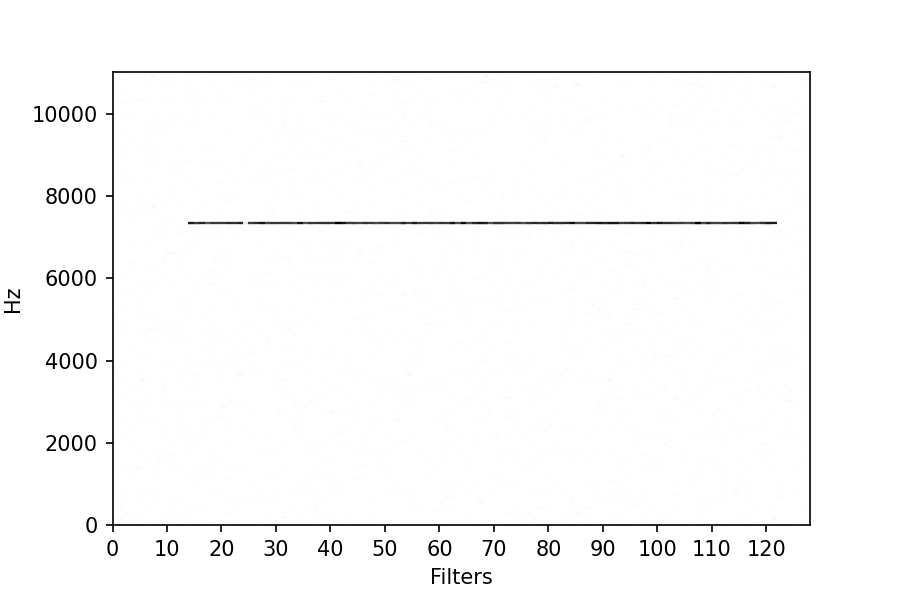
\includegraphics[width=.33\textwidth]{figs/magnatagatune/clmr_spectrum/epoch1490_layer0.png}}\hfill
    \subcaptionbox{CLMR$^{(4)}_{\mathrm{MTAT}}$\label{fig:1a}}{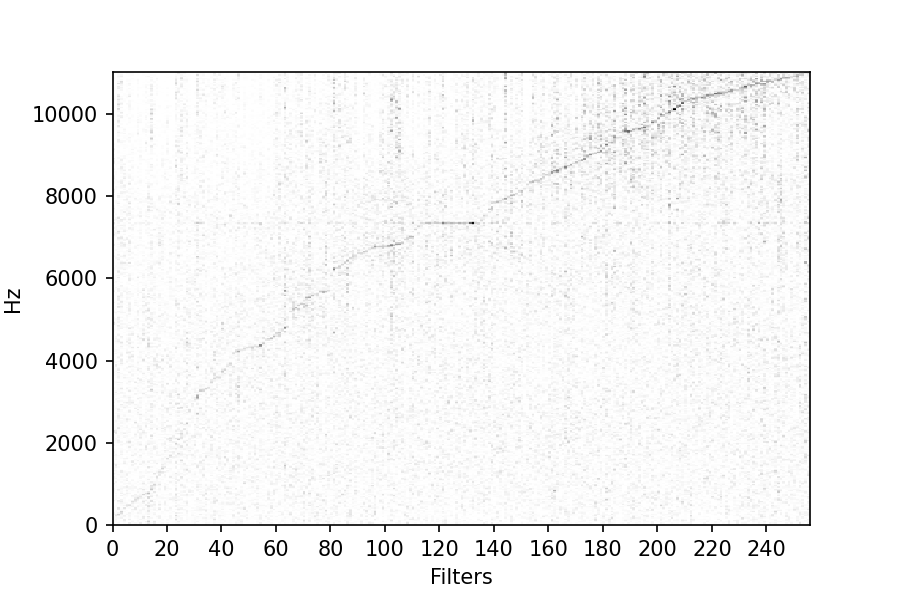
\includegraphics[width=.33\textwidth]{figs/magnatagatune/clmr_spectrum/epoch1490_layer3.png}}\hfill
    \subcaptionbox{CLMR$^{(6)}_{\mathrm{MTAT}}$\label{fig:1a}}{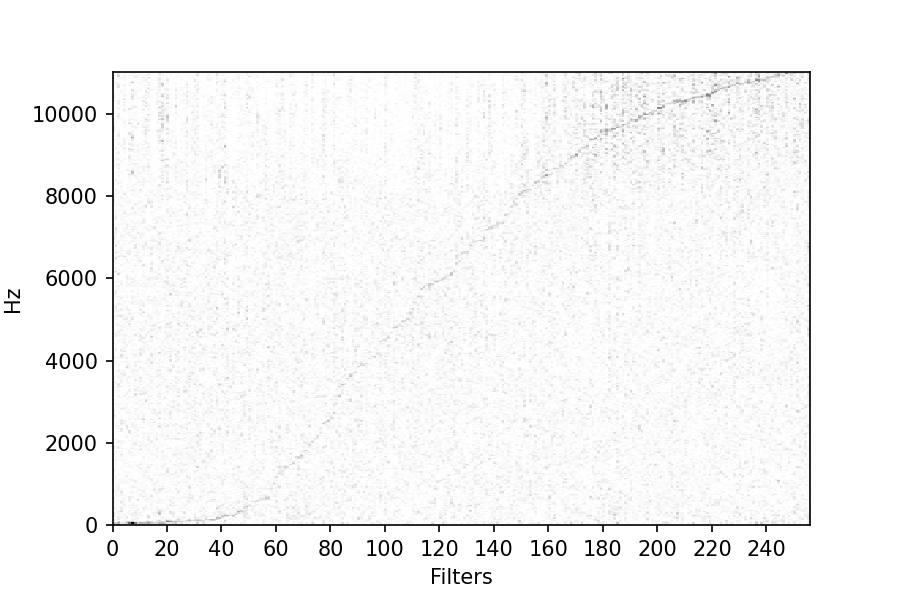
\includegraphics[width=.33\textwidth]{figs/magnatagatune/clmr_spectrum/epoch1490_layer5.png}}

    \subcaptionbox{CPC$^{(1)}_{\mathrm{MTAT}}$\label{fig:1a}}{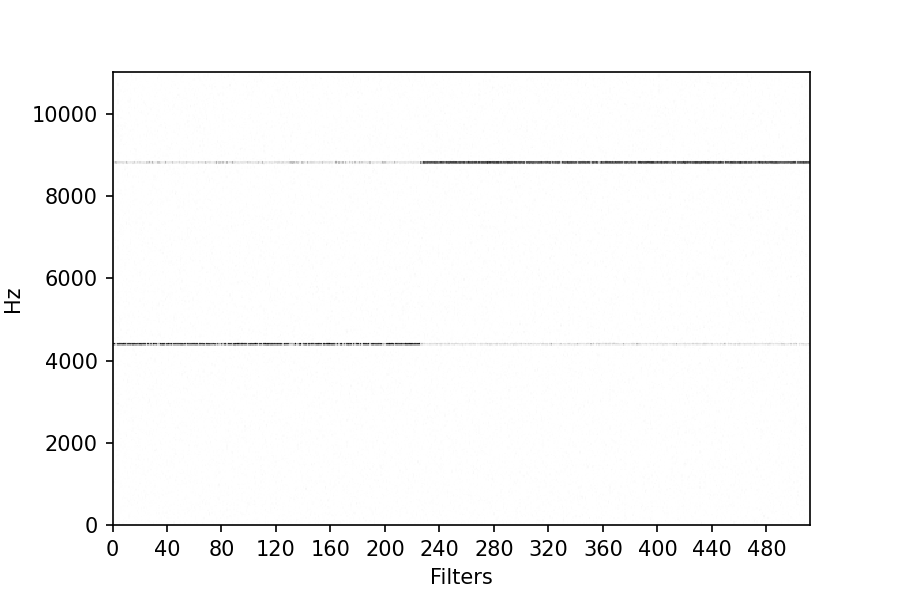
\includegraphics[width=.33\textwidth]{figs/magnatagatune/cpc_spectrum/epoch670_layer0.png}}\hfill
    \subcaptionbox{CPC$^{(4)}_{\mathrm{MTAT}}$\label{fig:1a}}{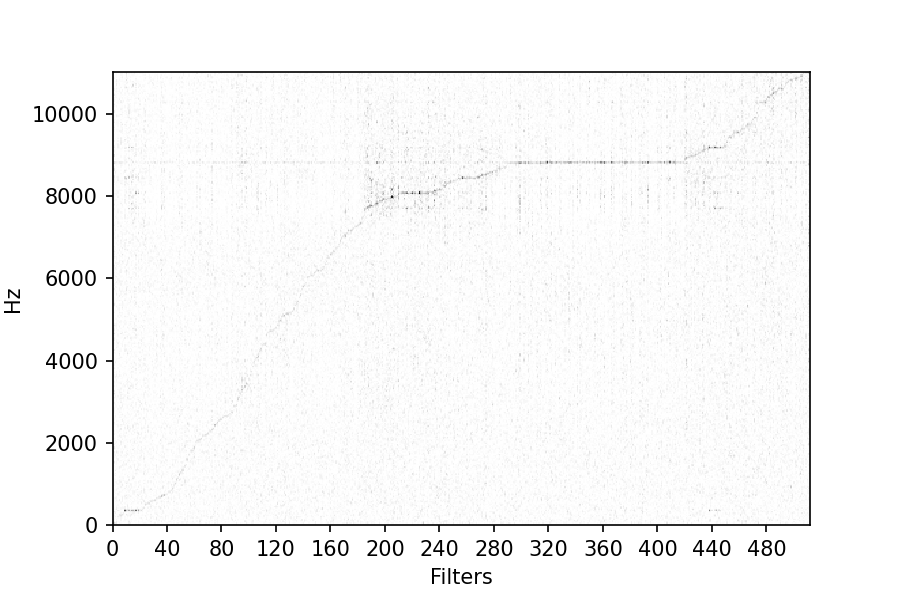
\includegraphics[width=.33\textwidth]{figs/magnatagatune/cpc_spectrum/epoch670_layer3.png}}\hfill
    \subcaptionbox{CPC$^{(6)}_{\mathrm{MTAT}}$\label{fig:1a}}{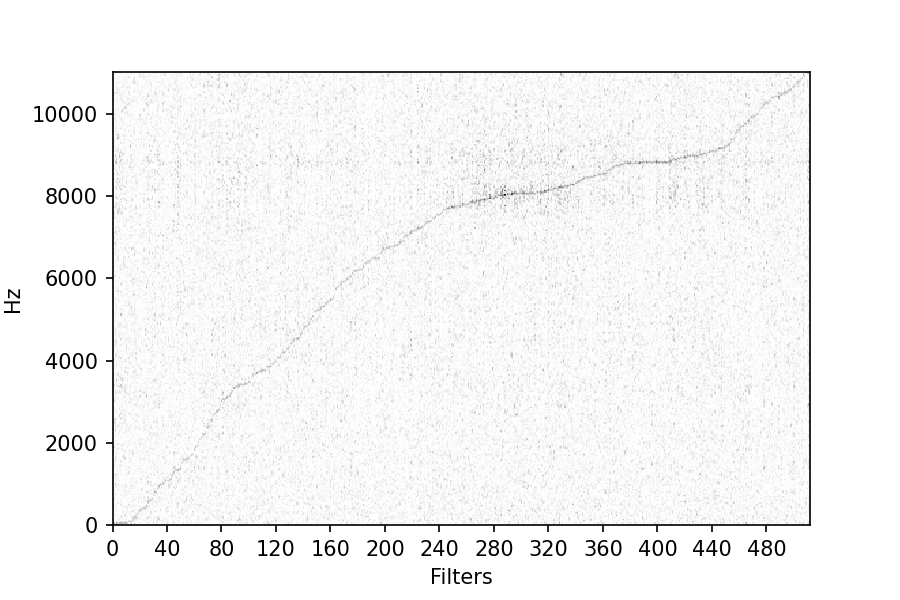
\includegraphics[width=.33\textwidth]{figs/magnatagatune/cpc_spectrum/epoch670_layer5.png}}

    \caption[][-3cm]{Normalised magnitude spectrum of the filters of the self-supervised models in the sample-level convolution layers, sorted by the frequency of the peak magnitude. Gradient ascent is performed on a randomly initialised waveform of 729 samples (close to typical frame size) and its magnitude spectrum is calculated subsequently. Each vertical line in the graph represents the frequency spectrum of a different filter. The first three images are taken from a pre-trained, converged CLMR model, the last three from a CPC model. Both are trained on the MagnaTagATune dataset.}
    \label{fig:filter_visualisation}
\end{figure}

\begin{figure}
    \centering
    \subcaptionbox{CLMR$^{(1)}_{\mathrm{Billboard}}$\label{fig:1a}}{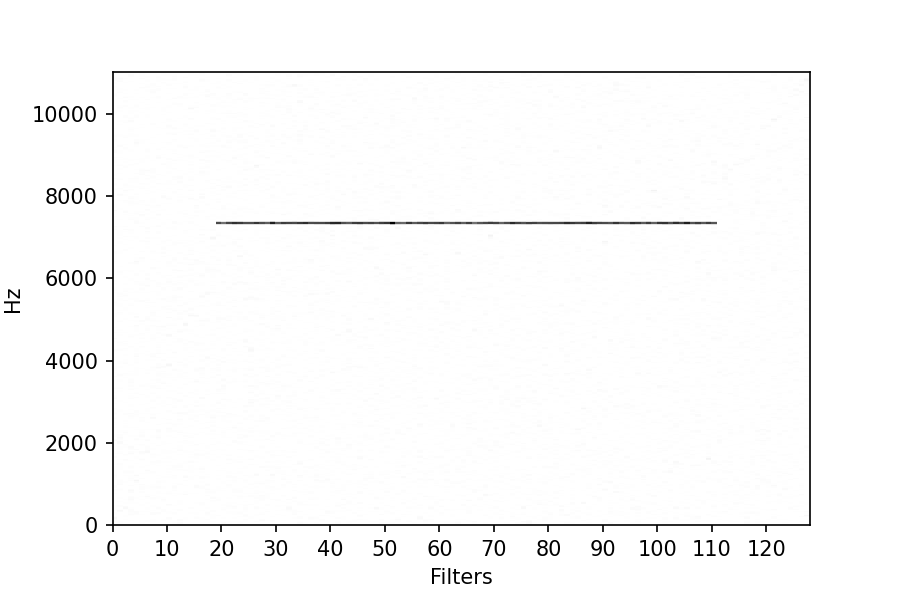
\includegraphics[width=.33\textwidth]{figs/billboard/clmr_spectrum/epoch1490_layer0.png}}\hfill
    \subcaptionbox{CLMR$^{(4)}_{\mathrm{Billboard}}$\label{fig:1a}}{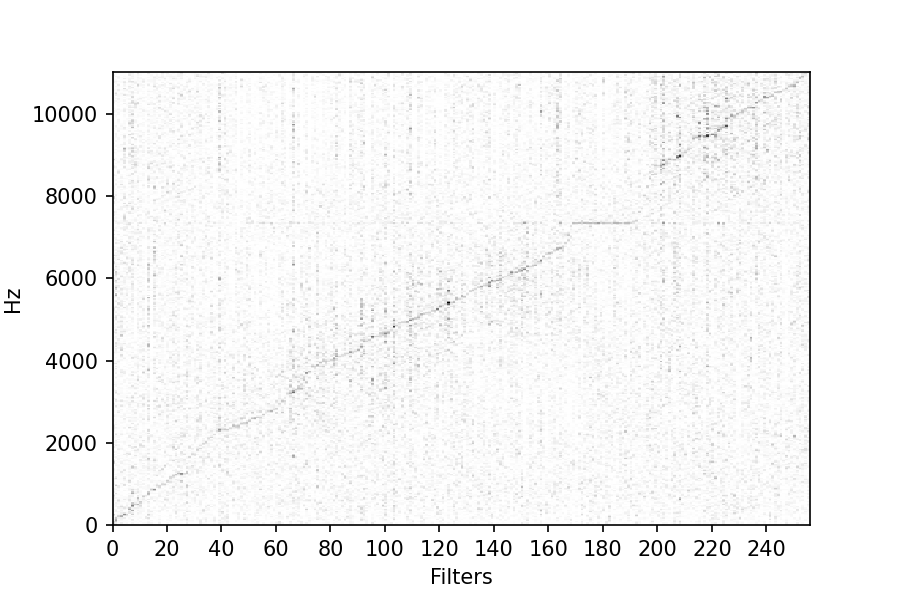
\includegraphics[width=.33\textwidth]{figs/billboard/clmr_spectrum/epoch1490_layer3.png}}\hfill
    \subcaptionbox{CLMR$^{(6)}_{\mathrm{Billboard}}$\label{fig:1a}}{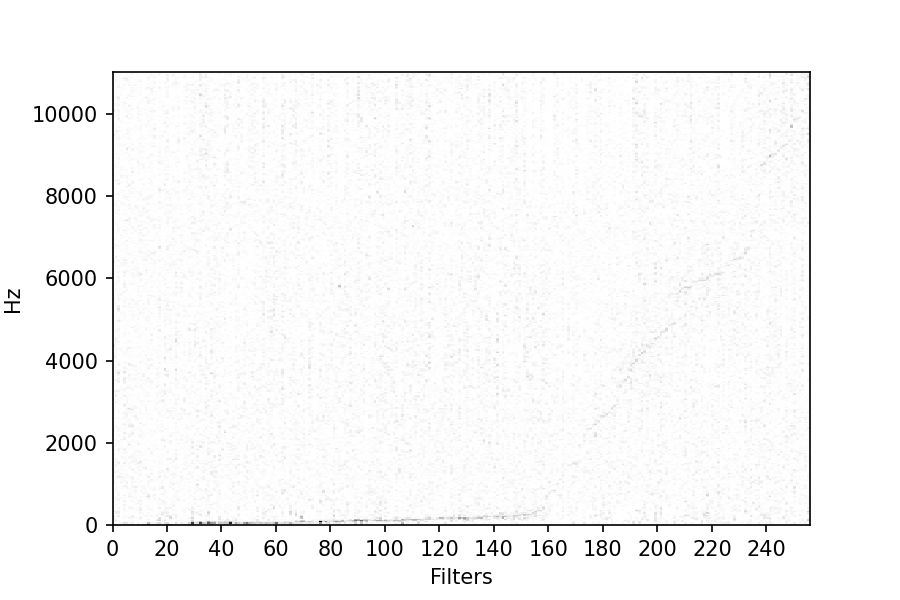
\includegraphics[width=.33\textwidth]{figs/billboard/clmr_spectrum/epoch1490_layer5.png}}

    \subcaptionbox{CPC$^{(1)}_{\mathrm{Billboard}}$\label{fig:1a}}{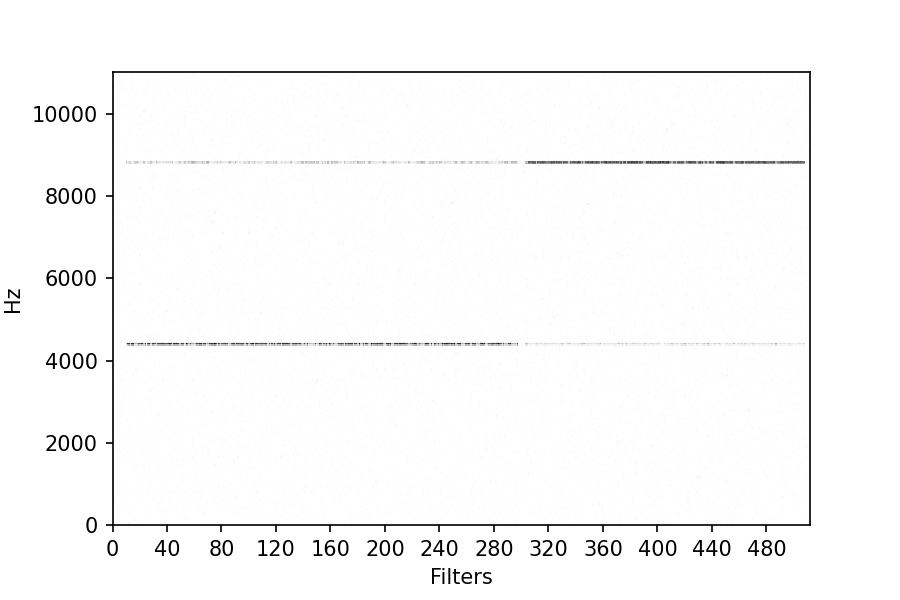
\includegraphics[width=.33\textwidth]{figs/billboard/cpc_spectrum/epoch1490_layer0.png}}\hfill
    \subcaptionbox{CPC$^{(4)}_{\mathrm{Billboard}}$\label{fig:1a}}{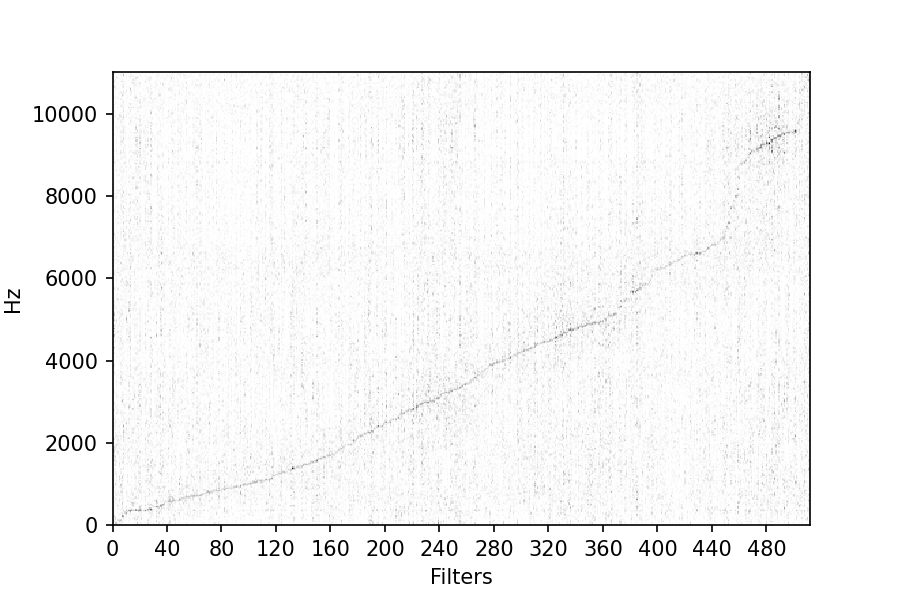
\includegraphics[width=.33\textwidth]{figs/billboard/cpc_spectrum/epoch1490_layer3.png}}\hfill
    \subcaptionbox{CPC$^{(6)}_{\mathrm{Billboard}}$\label{fig:1a}}{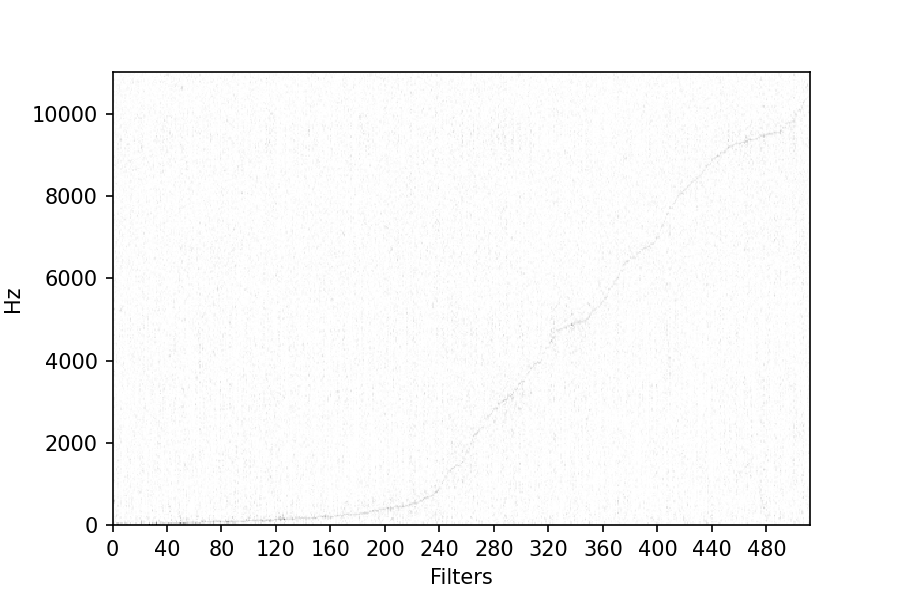
\includegraphics[width=.33\textwidth]{figs/billboard/cpc_spectrum/epoch1490_layer5.png}}
    \caption{Normalised magnitude spectra, generated using the method described in Figure \ref{fig:filter_visualisation}. These CLMR and CPC models were trained on the Billboard dataset}
    \label{fig:filter_visualisation_billboard}
\end{figure}

\begin{figure}
    \centering
    \includegraphics[width=\textwidth]{figs/samplecnn_filters.png}
    \caption{Normalised magnitude spectrum of filters from layers 1 - 6 of a fully end-to-end trained supervised SampleCNN network. Figure is taken from Figure 3 in \cite{lee2018samplecnn}.}
    \label{fig:samplecnn_filters}
\end{figure}


\section{Activations}
\label{sec:activations}
Figure \ref{fig:magnatagatune_activations} and \ref{fig:msd_activations} show the mean activations\footnote{We use the term "activations" to describe the values that are obtained from the last convolutional layer of the SampleCNN encoder, i.e., from the 512 filters, when predicting a segment of musical audio.} of the last convolutional block of the SampleCNN encoder for every music segment in the test set, for both the MagnaTagATune and Million Song Dataset respectively. In contrast to the MagnaTagATune activations, the last layer of the encoder from the Million Song Dataset activates more broadly for every track, indicating that the encoder responds more flatly. It is important to note that the feature numbers on the x-axis in Figures \ref{fig:magnatagatune_activations} and \ref{fig:msd_activations} do not correspond to the actual mean activation value - they show how many features were used in the last layer of the SampleCNN encoder. In the following paragraph, we describe a qualitative analysis that uses these activations.

\begin{marginfigure}
    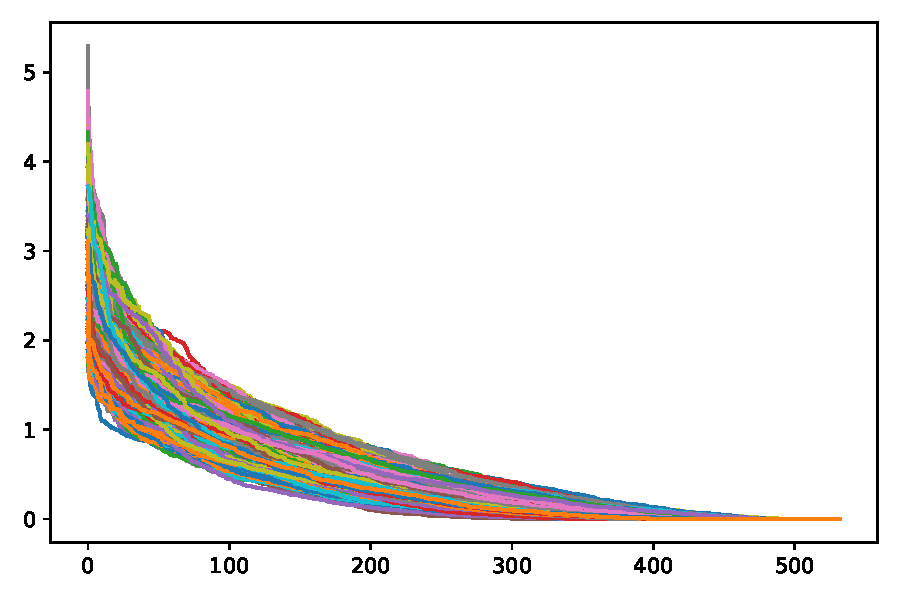
\includegraphics[width=\textwidth]{figs/activations.pdf}
    \caption{Mean activations of 512 features for every music segment, sorted by activation value. Extracted from the encoder of a converged CLMR model trained on the MagnaTagATune dataset.}
    \label{fig:magnatagatune_activations}
\end{marginfigure}

\begin{marginfigure}
    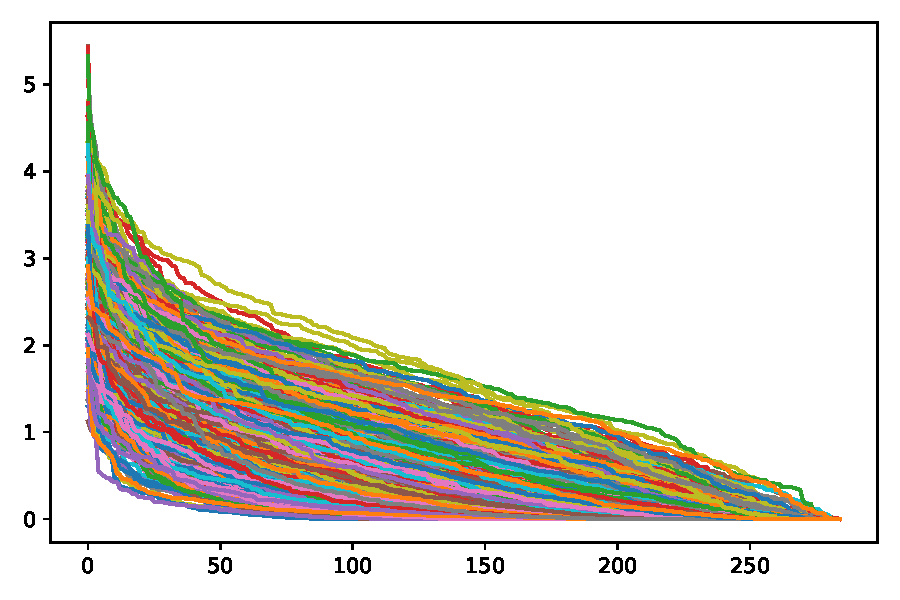
\includegraphics[width=\textwidth]{figs/activations_msd.pdf}
    \caption{Mean activations of 512 features for every music segment, sorted by activation value. Extracted from the encoder of a converged CLMR model trained on the Million Song Dataset.}
    \label{fig:msd_activations}
\end{marginfigure}

\section{Listening Experiment}
We have devised an interface which makes it easy to listen to music segments that were run through the CLMR model.
For any one of the 512 filters (i.e., features) in the last layer of the pre-trained SampleCNN encoder, we calculate the activations for each music segment.
This yields a table of 512 columns of features and $X$ sorted rows based on the activation value of filter.
\footnote{$X$ being the number of data points in the dataset's test set.}

We take the following, basic approach to qualitatively analyse the features learned by our self-supervised model:
\begin{itemize}
    \item We calculate the filter activations of the last convolution layer for all music segments in the test set, yielding a 512-dimensional feature vector for every segment.
    \item We plot these values in a sortable table and including the corresponding, listenable music segment.
    \item We choose a single feature from any of the 512 available, and sort the activation values in a descending order.
    \item We listen to the top-$N$ segments, and write down the sound qualities of those in the upper level (i.e., the first $N$).
\end{itemize}

A screenshot of the listening experiment interface is shown in Figure \ref{fig:listening_experiment}. We guided our listening experiment with factor analysis first. While this did not yield good results, we later used a manual approach described in paragraph \ref{sec:manual_interpretations}. We included the factor analysis paragraph for future improvement.

\section{Factor Analysis}
The following analysis is performed using a converged CLMR model that was pre-trained on the MagnaTagATune dataset.

A factor analysis is used to describe correlated variables using a lower number of unobserved variables, i.e., whether variations of many variables reflect those of fewer variables. To guide our listening experiment, we use varimax rotation on the fully connected 512-dimensional layer that is extracted from the linear (or MLP) head after fine-tuning has converged. We choose to use 3 components and subsequently sort each of the 512-dimensional feature vectors by their factor value per component. These are shown in Figure \ref{fig:varimax_rotation}. This gives us an indication which feature numbers are more closely related.

\begin{figure}[h]
    \centering
    \begin{subfigure}[b]{0.3\textwidth}
        \centering
        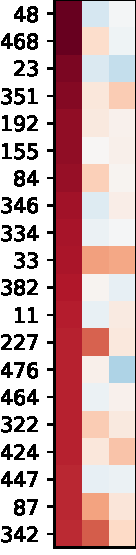
\includegraphics[width=\textwidth]{figs/varimax-magnatagatune-0.pdf}
        \caption{Component 1}
    \end{subfigure}
    \hfill
    \begin{subfigure}[b]{0.3\textwidth}
        \centering
        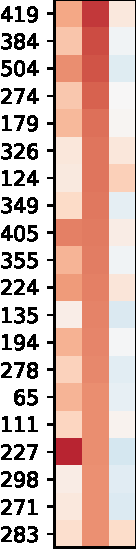
\includegraphics[width=\textwidth]{figs/varimax-magnatagatune-1.pdf}
        \caption{Component 2}
    \end{subfigure}
    \hfill
    \begin{subfigure}[b]{0.3\textwidth}
        \centering
        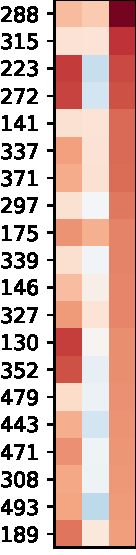
\includegraphics[width=\textwidth]{figs/varimax-magnatagatune-2.pdf}
        \caption{Component 3}
    \end{subfigure}
    \caption[][24pt]{Varimax rotation of 3 components on 512 factors (features) on a pre-trained CLMR model on the MagnaTagATune dataset. The figure shows the 20 strongest factors per component.}
    \label{fig:varimax_rotation}
\end{figure}

After listening to segments that highly activate among the relating features obtained from sorting the factors for each component using varimax, we quickly found that it was biased toward grouping loud, techno/(hard-)rock music together for every single component (i.e., for components 1 - 3). To analyse a possible reason for this behavior, we plotted the number of tags in the top-10 activating segments for every feature number in the 512-dimensional feature vector. This is shown in Figure \ref{fig:tag_frequency}. It shows the more dominantly present tags that are predicted for every feature number, e.g., `techno, `rock', `beat', `loud', `dance'. Most features respond highly to these tags, while other tags like `vocal' or `flute' occur less often. These results do not simply translate to the overall tag frequency: the `guitar' and `classical' tags occur more in the dataset, but show less activations overall than `techno' or `rock'.

While the Factor Analysis grouped together a single, dominant spectral feature, i.e., loudness, and while time is a constraint on the extensivity of this qualitative analysis, we resorted to an easier, but manual intepretation method using out-of-dataset data.

\begin{figure*}[h]
    \centering
    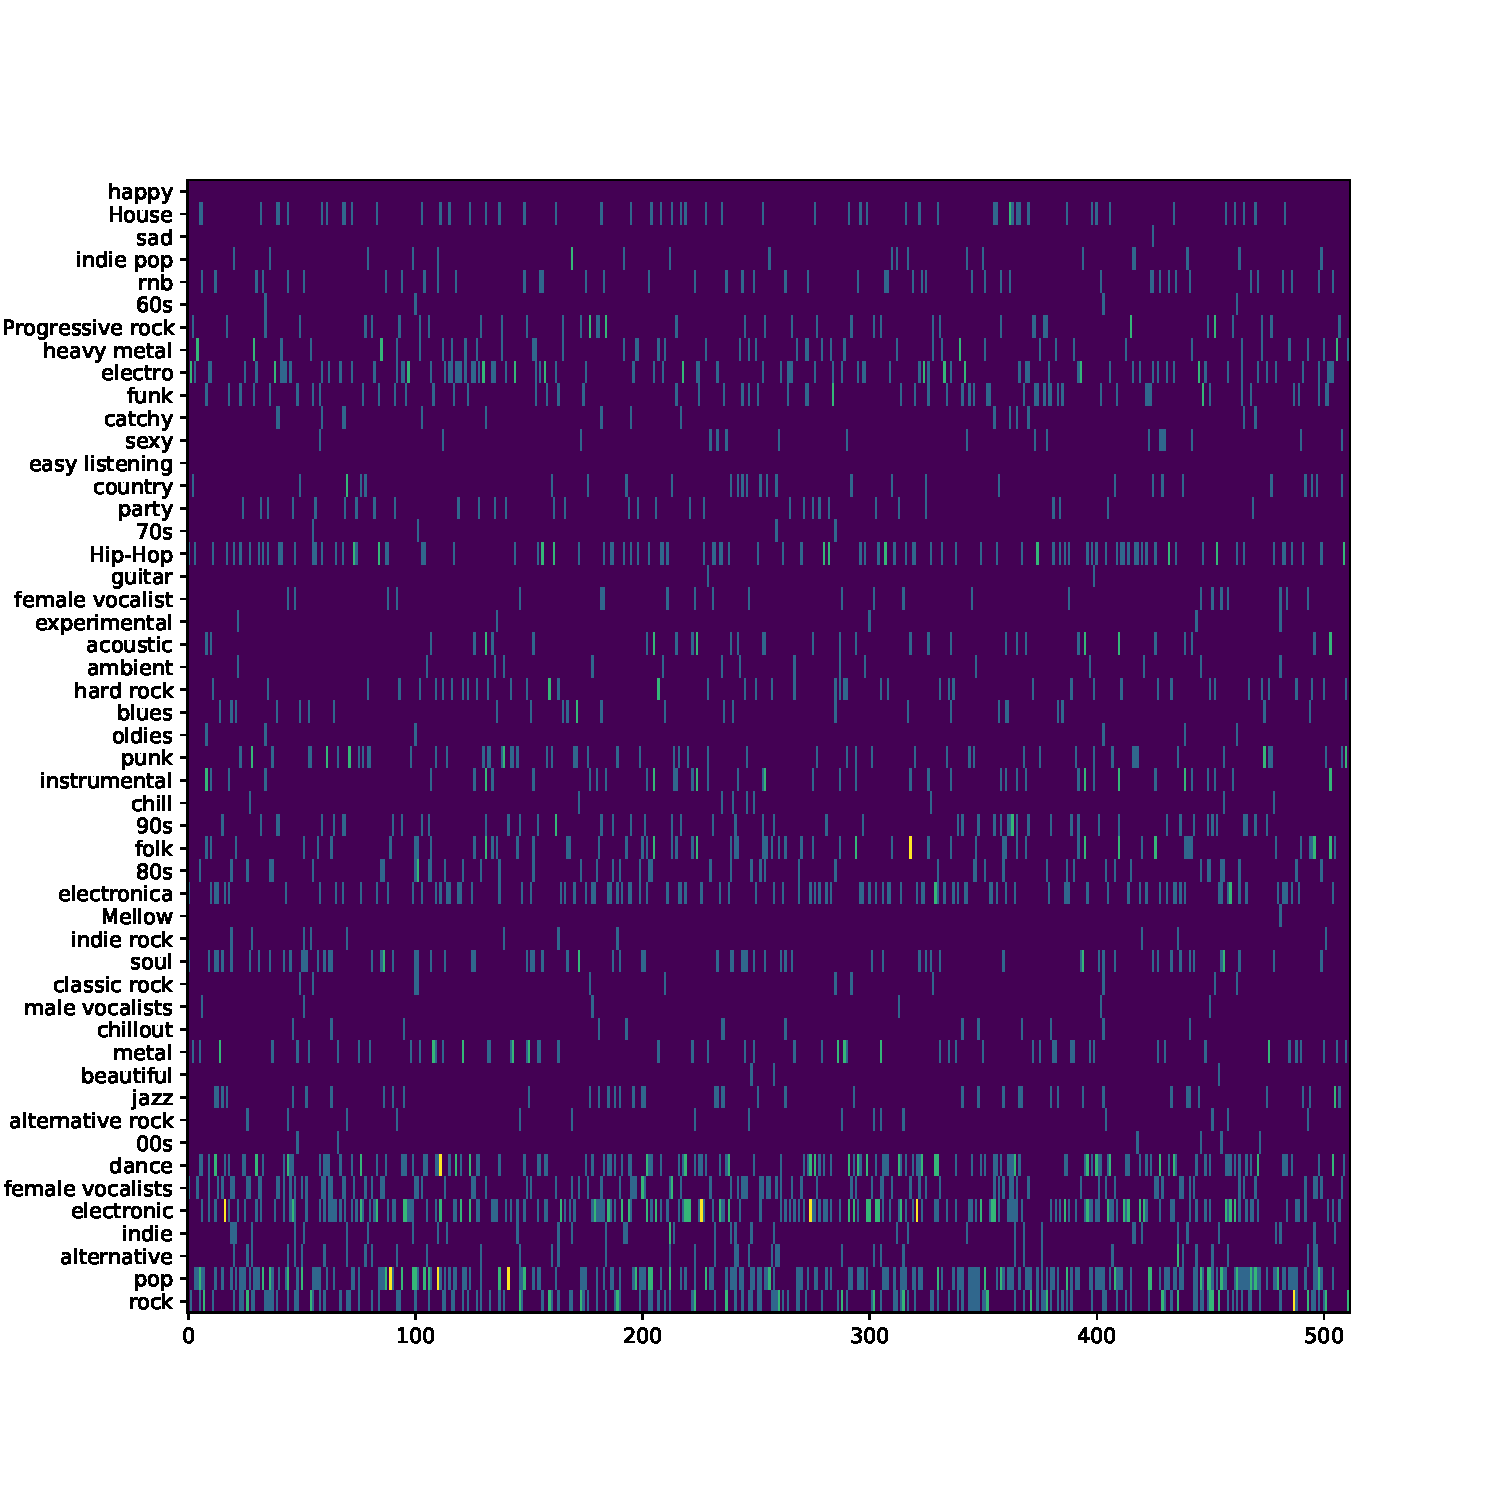
\includegraphics[width=\textwidth]{figs/features_tags_frequency.pdf}
    \caption{Occurrence of tags for the 100 most activating segments for each feature number. Purple indicates low, yellow indicates a high frequency.}
    \label{fig:tag_frequency}
\end{figure*}


\section{Out-of-domain Generalisation}\label{sec:manual_interpretations}
To evaluate whether certain features respond to similar spectral qualities, we process both the MagnaTagATune dataset, which the model was pre-trained on, and the Million Song Dataset through the encoder network. In this way, we are able to determine the \textit{out-of-domain generalisation} of the self-supervised model, i.e., is it able to learn features that describe similar sonic qualities of music originating from an entirely different library of music. We extract a 512-dimensional feature vector from the last SampleCNN filters for every segment (as described in Section \ref{sec:activations}), and evaluate whether the same filters respond to the same sonic qualities present in the music segments.

For example, we evaluate whether filter number $412$ highly activates on segments of slow-paced jazz music from both the MagnaTagATune and Million Song Dataset, or not. We describe each feature using sound qualities, e.g., in terms of the frequency spectrum, loudness, and ADSR qualities.\footnote{The attack, decay, sustain, release of the sound.} The filter numbers are pickled by manually listening to the most activating segments of the chosen filter and, when those musical pieces are sufficiently coherent, we listen to the most activating out-of-domain segments of the same filter.

\subsection*{Filter \#51}
\paragraph{MagnaTagATune}
Slow, vocal, string and flute instruments, accompanied by either harpsichord or guitar.
\paragraph{Million Song Dataset}
Slow, vocal accompanied by guitar. Some segments are up-paced jazz, but those recordings contain a lot of noise.

\subsection*{Filter \#61}
\paragraph{MagnaTagATune}
Loud, distorted guitars, vocals, heavy beat, snappy percussion and bass
\paragraph{Million Song Dataset}
Loud, heavy distorted guitars, hip-hop rapping vocals, percussive bass.

\subsection*{Filter \#76}
\paragraph{MagnaTagATune}
Slow string music, vocal, classical, and solo flute, slow attack, not "plucky".

\paragraph{Million Song Dataset}
Jazz and blues music and some ambient music containing pad sounds (i.e., very slow attack, long decay/sustain/release). The jazz band's brass section plays less "stabby" - but more loose. There is some string music, but overall the sound quality is more slow-moving than fast and pluck-sounding.


\subsection*{Filter \#80}
\paragraph{MagnaTagATune}
Very noisy, the full frequency spectrum can be heard, i.e., low bass notes to high notes. You can clearly hear the ambience of the room due to the "breathy" character of the recording.

\paragraph{Million Song Dataset}
More ambient, you can hear many textures in any register of the frequency spectrum. It is sometimes atonal. The sounds are often slowly moving, and again, the recording is very "breathy".


\subsection*{Filter \#105}
\paragraph{MagnaTagATune}
Most recordings contain a plucked or strummed, solo acoustic guitar. Both low- and higher-pitched notes are strummed or plucked in the recordings, and some contain additional instruments like strings and vocals. The guitar is, however, the main instrument. There are two segments of techno music, but both have a very noisy character, i.e., it is a low quality recording. 

\paragraph{Million Song Dataset}
All recordings contain strummed or plucked acoustic guitars, which have a dominant presence in every mix. Most recordings also contain vocals and additional percussive instruments. There is a single ambient recording among all the guitar-heavy music segments.


\subsection*{Filter \#130}
\paragraph{MagnaTagATune}
The recordings contain heavily distored guitars,  compressed singing and heavily processed drums. They have a loud character, e.g., rock, metal and heavy metal, and their frequency spectrum is mostly active in the low-mid range.

\paragraph{Million Song Dataset}
All recordings are either of punk, heavy metal or hard rock music. They are loud and the dominant frequencies are in the low- to mid-range. Again, all instruments are heavily processed in a similar fashion to aforedescribed distortion and compression mixing techniques.


\subsection*{Filter \#400}
\paragraph{MagnaTagATune}
All recordings contain one or more vocalists that are dominantly present in the mix. Some recordings contain more reverb than others - but the vocals are always in the foreground of the mix. The singing style of these recordings are opera and non-western, featuring both male and female vocalists.

\paragraph{Million Song Dataset}
The recordings contain jazz, hip-hop, "old classics" and 60s music. Every recording contains at least one vocalist who is in the foreground of the mix. They are accompanied by a range of backing tracks, e.g., a strong beat to a softly playing string section.


\subsection*{Filter \#80}
\paragraph{MagnaTagATune}

\paragraph{Million Song Dataset}



\begin{figure*}[h]
    \centering
    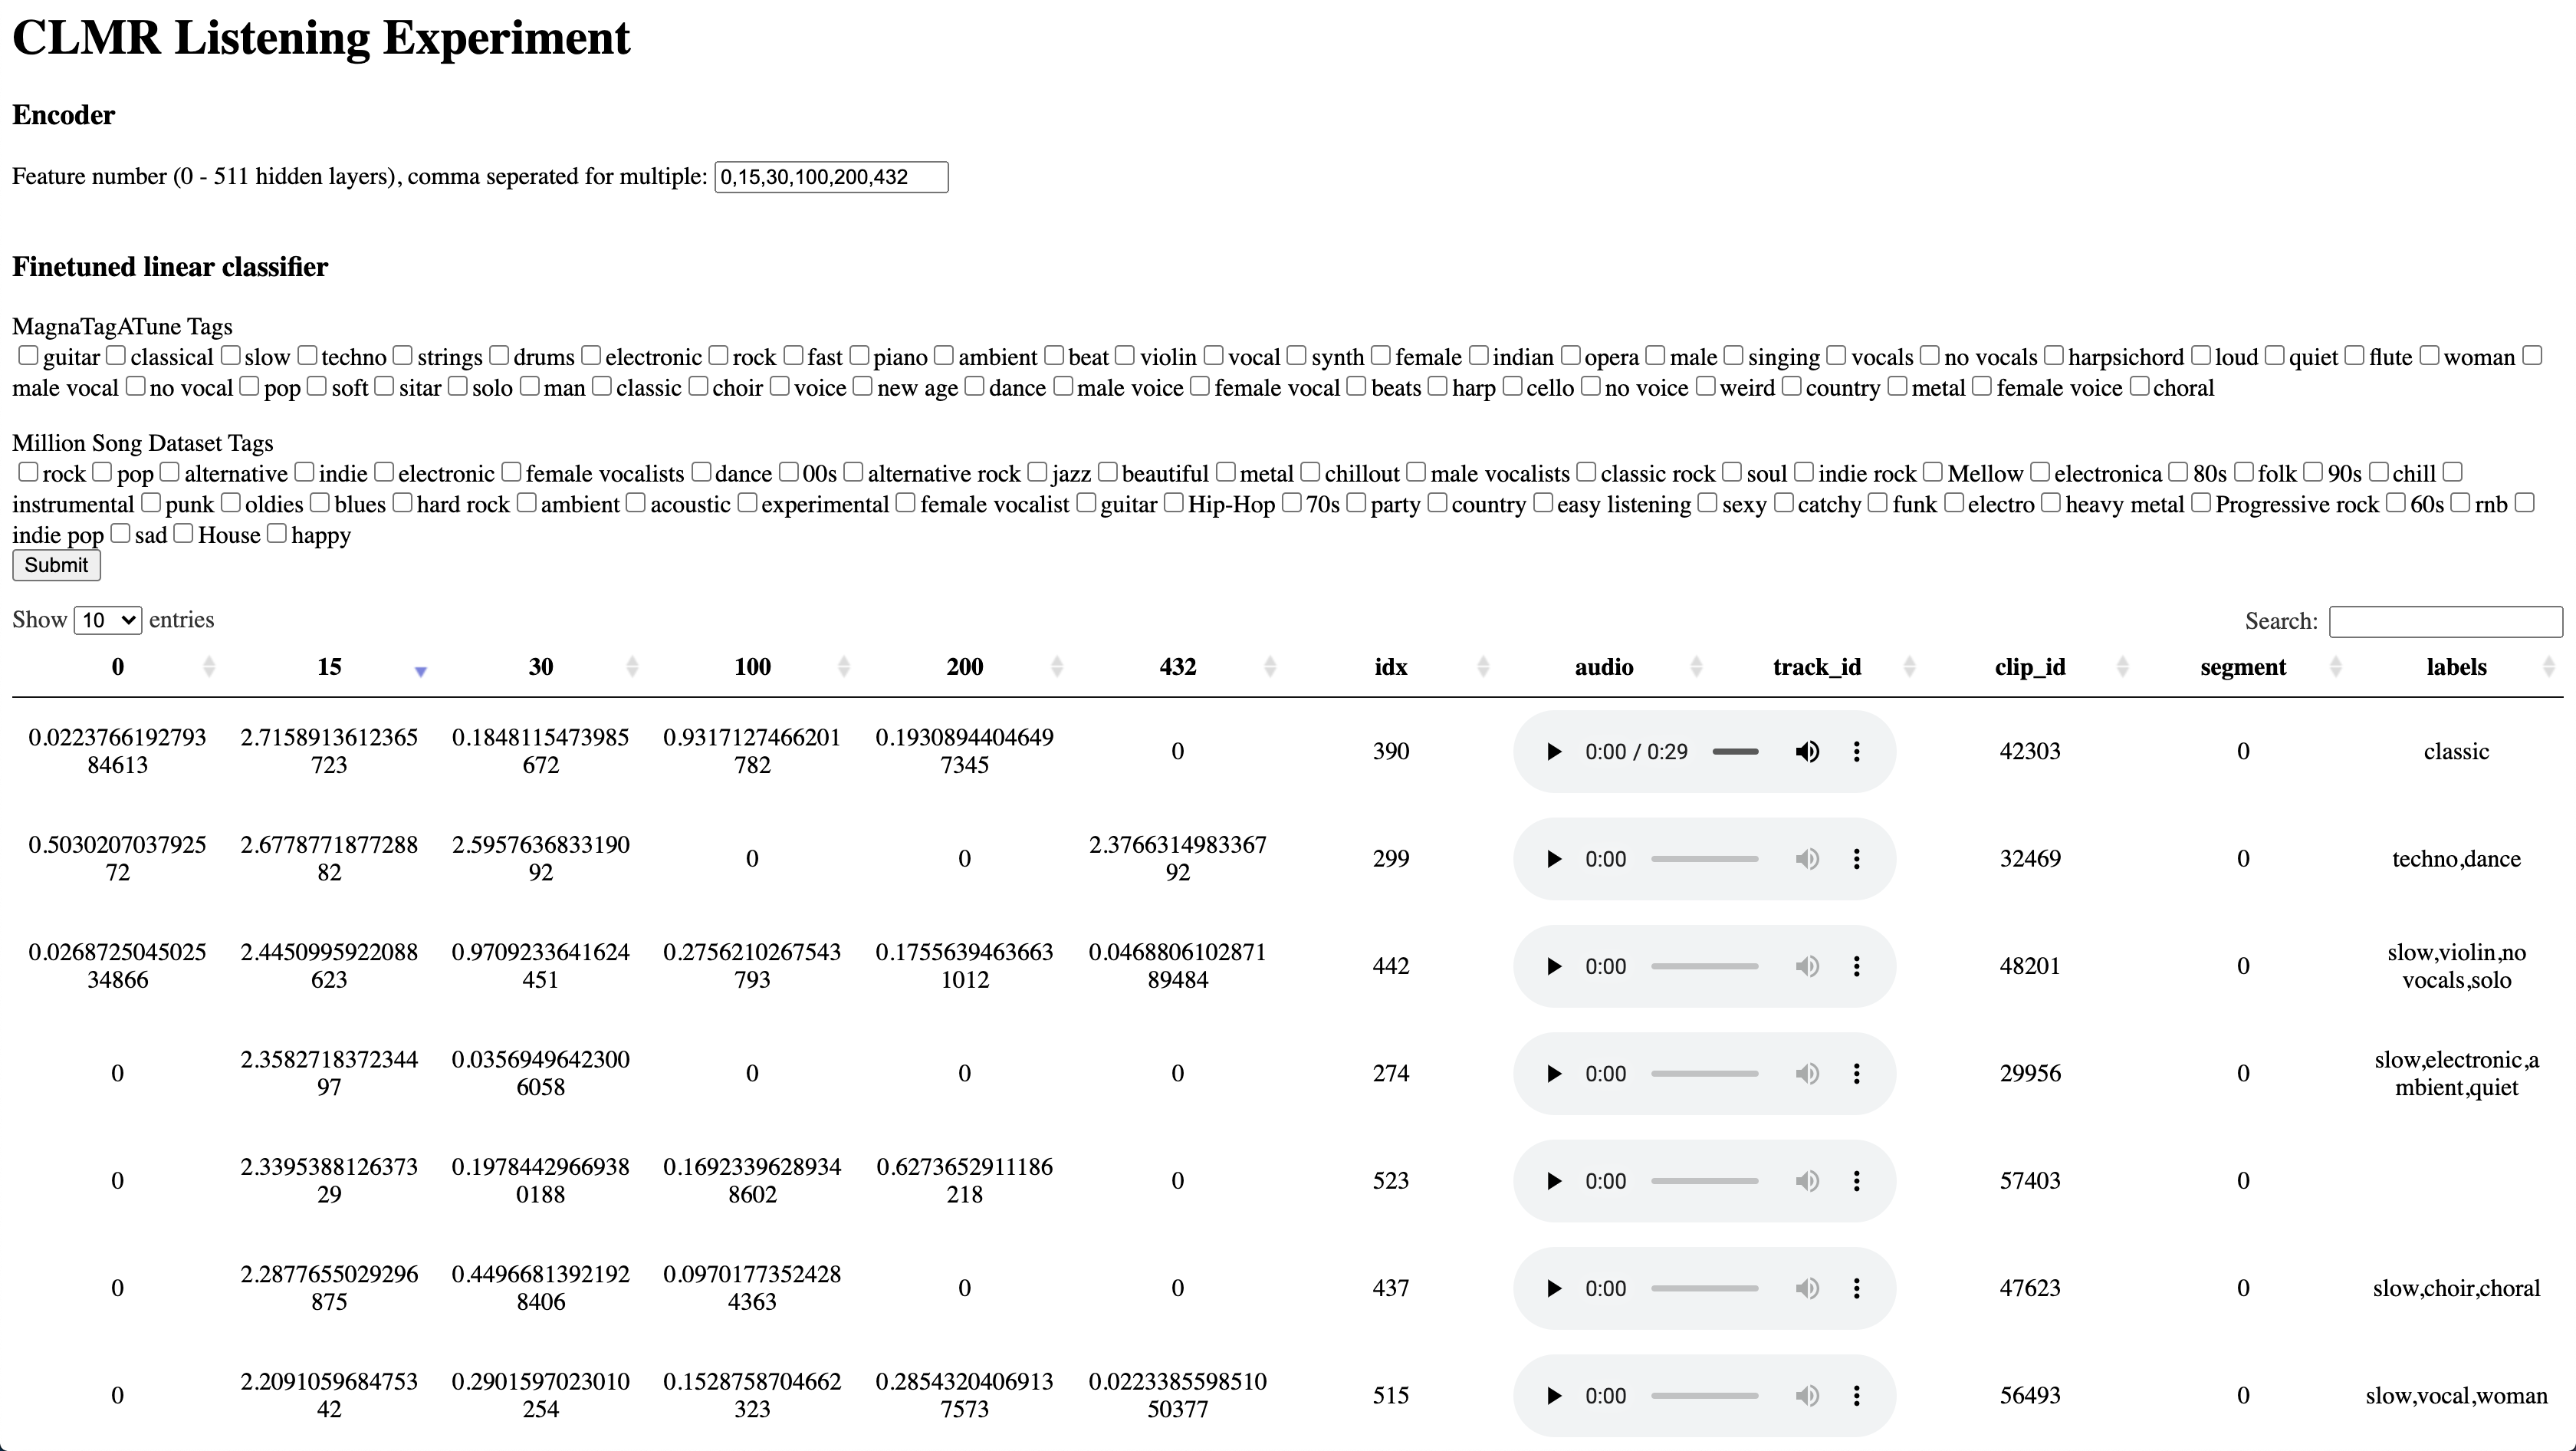
\includegraphics[width=\textwidth]{figs/listening_experiment.png}
    \caption{Screenshot of the listening experiment interface.}
    \label{fig:listening_experiment}
\end{figure*}

\section{Listenable Explanations}
Recently, a method based on Local Interpretable Model-agnostic Explanations was published that uses source separation to reconstruct the audio from a representation to produce a listenable explanation \cite{haunschmid2020audiolime}. The pre-trained encoder and fine-tuned (linear) head from the CLMR model are used in the audioLIME method to provide several examples to listen whether the model makes sensible predictions, i.e., what part of the fragment of audio it is focussing on when making a prediction. \footnote{URL}.